\documentclass[english, xcolor=dvipsnames, aspectratio=169]{beamer}
% packages
%----------------------------------------------------------------------------------------
%	PACKAGES AND OTHER DOCUMENT CONFIGURATIONS
%----------------------------------------------------------------------------------------

\documentclass[
	11pt, % Set the default font size, options include: 8pt, 9pt, 10pt, 11pt, 12pt, 14pt, 17pt, 20pt
	%t, % Uncomment to vertically align all slide content to the top of the slide, rather than the default centered
	%aspectratio=169, % Uncomment to set the aspect ratio to a 16:9 ratio which matches the aspect ratio of 1080p and 4K screens and projectors
]{beamer}

\graphicspath{{../../imgs/}{{../../imgs/04_Classification}}} % Specifies where to look for included images (trailing slash required)

\usepackage{booktabs} % Allows the use of \toprule, \midrule and \bottomrule for better rules in tables

\usepackage[T1]{fontenc}
\usepackage{mathptmx}
% Define colors variables
% Define colors variables
\definecolor{red}{rgb}{0.631, 0.094, 0.094} % primary color
\definecolor{grey}{rgb}{0.3686, 0.5255, 0.6235} % secondary color
\definecolor{blue}{rgb}{0.27, 0.509, 0.705} % primary color

% Title page
\title{Neural networks}
\author{Blanca Cano Camarero}
\institute{Universidad Autónoma de Madrid}

  % logo of my university
  \titlegraphic{
    
\includegraphics[width=0.4\textwidth]{logos/uam-iic.jpeg}
}

% Date
\day=16\relax
\month=12\relax
\year=2022\relax

% Color template 
\newcommand{\bgcolor}{blue}
% Beamer parameters
% Set theme palette colors
\setbeamercolor{palette primary}{bg=\bgcolor,fg=white}
\setbeamercolor{palette secondary}{bg=\bgcolor,fg=white}
\setbeamercolor{palette tertiary}{bg=\bgcolor,fg=white}
\setbeamercolor{palette quaternary}{bg=\bgcolor,fg=white}
% strucure means itemize, enumerate, etc
\setbeamercolor{structure}{fg=\bgcolor} 

% Set bibliography colors
\setbeamercolor{bibliography item}{fg=\bgcolor}
\setbeamercolor{bibliography entry author}{fg=black}
\setbeamercolor{bibliography entry title}{fg=black}
\setbeamercolor{bibliography entry location}{fg=black}
\setbeamercolor{bibliography entry note}{fg=black}
% Replaces book icon in bibliography with enumeration
\setbeamertemplate{bibliography item}{[\theenumiv]}

% Table of contents style
% \setbeamertemplate{section in toc}[sections numbe\bgcolor]
% \setbeamertemplate{subsection in toc}[subsections numbe\bgcolor]
\setbeamertemplate{section in toc}[circle]
\setbeamertemplate{subsection in toc}[ball unnumbe\bgcolor]

% Header with navigation bar
\setbeamertemplate{headline}
{
    \leavevmode
    \hbox{
    \begin{beamercolorbox}[wd=\paperwidth,ht=2.5ex,dp=1.125ex]{palette quaternary}
    \insertsectionnavigationhorizontal{\paperwidth}{}{\hskip0pt plus1filll}
    \end{beamercolorbox} 
    }
}
% Footer with custom caption
\setbeamertemplate{footline}
{
    \leavevmode
    \hbox{
    \begin{beamercolorbox}[wd=.33\paperwidth,ht=2.6ex,dp=1ex,center]{palette quaternary}
    \usebeamerfont{author in head/foot}\insertshortauthor\hspace*{1ex}
    \end{beamercolorbox}
    \begin{beamercolorbox}[wd=.33\paperwidth,ht=2.6ex,dp=1ex,center]{palette quaternary}
    \usebeamerfont{institute in head/foot}\insertshortinstitute
    \end{beamercolorbox}
    \begin{beamercolorbox}[wd=.33\paperwidth,ht=2.6ex,dp=1ex,center]{palette quaternary}
    \insertframenumber{} / \inserttotalframenumber
    \end{beamercolorbox}}
    \vskip0pt
}

%% Custom commands
%% ===============

%% Special characters for number sets, e.g. real or complex numbers.
\newcommand{\C}{\mathbb{C}}
\newcommand{\K}{\mathbb{K}}
\newcommand{\N}{\mathbb{N}}
\newcommand{\Q}{\mathbb{Q}}
\newcommand{\R}{\mathbb{R}}
\newcommand{\Z}{\mathbb{Z}}
\newcommand{\X}{\mathbb{X}}

%% Fixed/scaling delimiter examples (see mathtools documentation)
\DeclarePairedDelimiter\abs{\lvert}{\rvert}
\DeclarePairedDelimiter\norm{\lVert}{\rVert}

%% Use the alternative epsilon per default and define the old one as \oldepsilon
\let\oldepsilon\epsilon
\renewcommand{\epsilon}{\ensuremath\varepsilon}

%% Also set the alternate phi as default.
\let\oldphi\phi
\renewcommand{\phi}{\ensuremath{\varphi}}

\newcommand{\logo}[1][\textwidth]{\resizebox{#1}{!}{
\includegraphics{logos/uam-iic.jpeg}}}




\begin{document}

\frame{\titlepage}

% Complete table of contents (ToC)
% \customToC{hideallsubsections}{}
%\customToC{}{}

%%%%%%% add sections here %%%%%%%
% Section name and highlighted ToC
%\renewcommand{\sectiontitle}{Introduction}
%\section{\sectiontitle}
%\customToC{currentsection,hideothersubsections}{}

% Section name and highlighted ToC
%\renewcommand{\subsectiontitle}{What is machine learning?}
%\subsection{\subsectiontitle}


\begin{frame}{Overview}
  \tableofcontents
\end{frame}
%%%% Work summary 
\section{Article data}

\begin{frame}
    \frametitle{Understanding the difficulty of training deep feedforward neural networks}
      \begin{itemize}
        \item Authors: Xavier Glorot and Yoshua Bengio.
        \item Publication year: 2010.
        \item Conference: Proceedings of the thirteenth international conference on artificial intelligence and statistics.
        \item Cited by: 19886 (I have found is quite a lot!) 
      \end{itemize}
      Reference: \cite{Understanding_the_difficulty_of_training_deep_feedforward_neural_networks}
\end{frame}

\section{Abstract}
\begin{frame}
  \frametitle{Abstract}

  \textbf{Context}
  \begin{itemize}
    \item Before 2006 deep multilayer neural networks were not successfully trained. 
    \item But after, by new initialization or training mechanisms experimental results showed the superiority of deeper vs less deep architectures. 
  \end{itemize}

  \textbf{Article objetive}
  \begin{itemize}
    \item Understand why standard gradient descent from random initialization is doing so poorly with deep neural networks. 
  \end{itemize}

  %\textbf{Motivation}
 % \begin{itemize}
  %  \item Design better algorithm. 
  %\end{itemize}
  
\end{frame}
    
\begin{frame}
  
  \textbf{Experiments}
  \begin{itemize}
    \item Observe the influence of the non-linear activations functions:
    \begin{itemize}
      \item Logistic sigmoid activation is unsuited for deep networks for deep networks with random initialization due to its mean value, which can drive especially the \textbf{top hidden layer into saturation}. 
      \item Saturated units can move out of saturation by themselves, albeit slowly (and explain the plateaus sometimes seen when training neural networks). 
      \item Found a new non-linearity that saturares less can often be beneficial. 
  \end{itemize}
    \item They \textbf{study how activations and gradients vary across layers and during training}, with the idea that training may be more difficult when the singular values of the Jacobian associated with each layer are far from one. 
    \item They proposed a new initialization scheme that brings substantially faster convergence. 
  \end{itemize}
  
\end{frame}

\section{Art state}

\begin{frame}
  \frametitle{Art state}

\end{frame}

\section{Experimental setting and Datasets}
\begin{frame}
  \frametitle{Experimental setting and Datasets}
   \textbf{Online learning on a synthetic images dataset: \textbf{Shapeset- 3} $\times 2$ dataset.}
  \begin{itemize}
    \item Focus on optimization issues rather than on the small-sample regularization effects.
    \item  The learner tries to predict which objects (parallelogram, triangle, or elipse) are presented, and one or two objects can be present yield into 9 possible classification.  
  \end{itemize}

  \begin{figure}[t]
    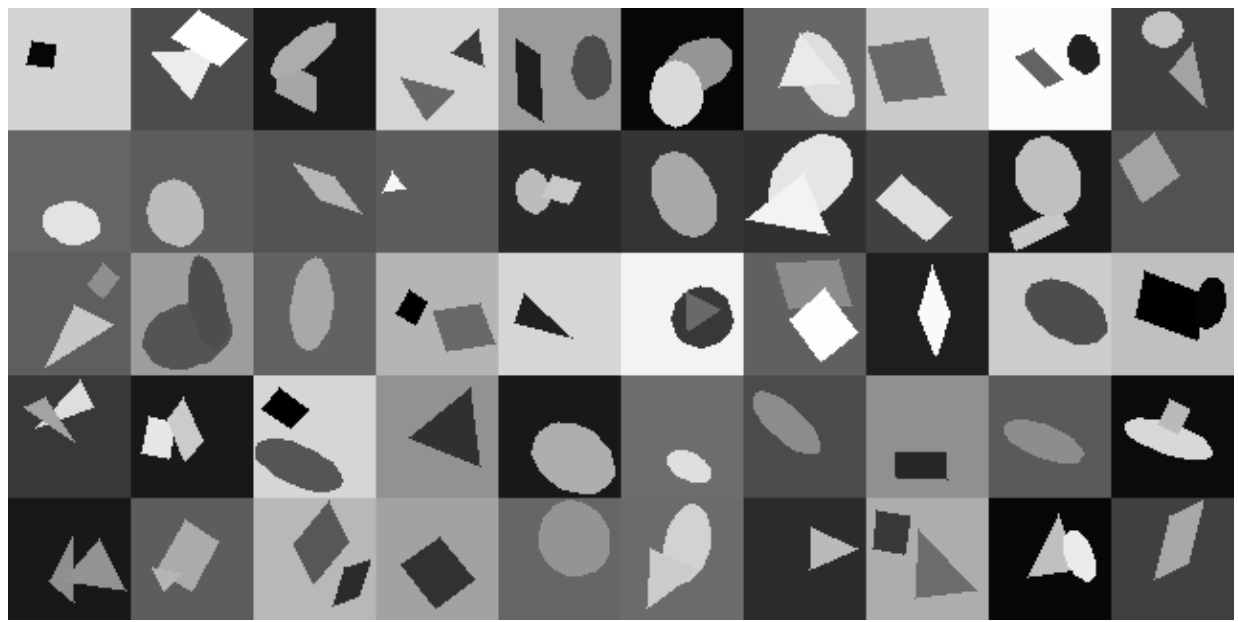
\includegraphics[height=0.4\textheight]{05_Understanding_deep_learning/shapeset-3x2.png}
    \centering
\end{figure}

\end{frame}

\begin{frame}
  \frametitle{Finite Datasets}

  \begin{itemize}
    \item The MNIST digits. 
    \begin{itemize}
      \item 50,000 training images,
      \item 10,000 validations images.
    \end{itemize}
    \item CIFAR-10 labeled subset of the tiny images. 
    \begin{itemize}
      \item 50,000 training images,
      \item 10,000 validations images,
      \item 10 classes corresponding to he main object:  airplane, au- tomobile, bird, cat, deer, dog, frog, horse, ship, or truck.
      \item Classes are balanced. 
    \end{itemize}

    \item Small-ImageNet. 
   \begin{itemize}
      \item 90,000 training images,
      \item 10,000 validations images,
      \item 10 classes corresponding to he main object: reptiles, vehicles, birds, mammals, fish, furniture, instruments, tools, flowers and fruits.
      \item Classes are balanced. 
    \end{itemize}
  \end{itemize}

\end{frame}

\begin{frame}
  \begin{figure}
    \centering
    \begin{subfigure}[b]{0.3\textwidth}
        \centering
        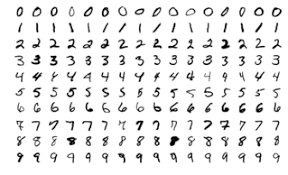
\includegraphics[width=\textwidth]{05_Understanding_deep_learning/MNIST.png}
        \caption{MNIST}
        \label{fig:y equals x}
    \end{subfigure}
    \hfill
    \begin{subfigure}[b]{0.3\textwidth}
        \centering
        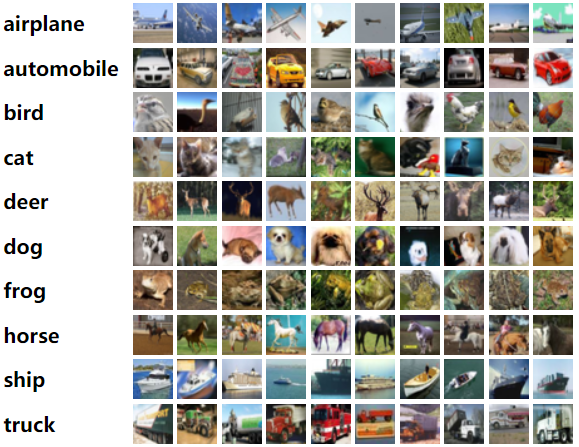
\includegraphics[width=\textwidth]{05_Understanding_deep_learning/CIFAR-10.png}
        \caption{CIFAR-10}
        \label{fig:three sin x}
    \end{subfigure}
    \hfill
    \begin{subfigure}[b]{0.3\textwidth}
        \centering
        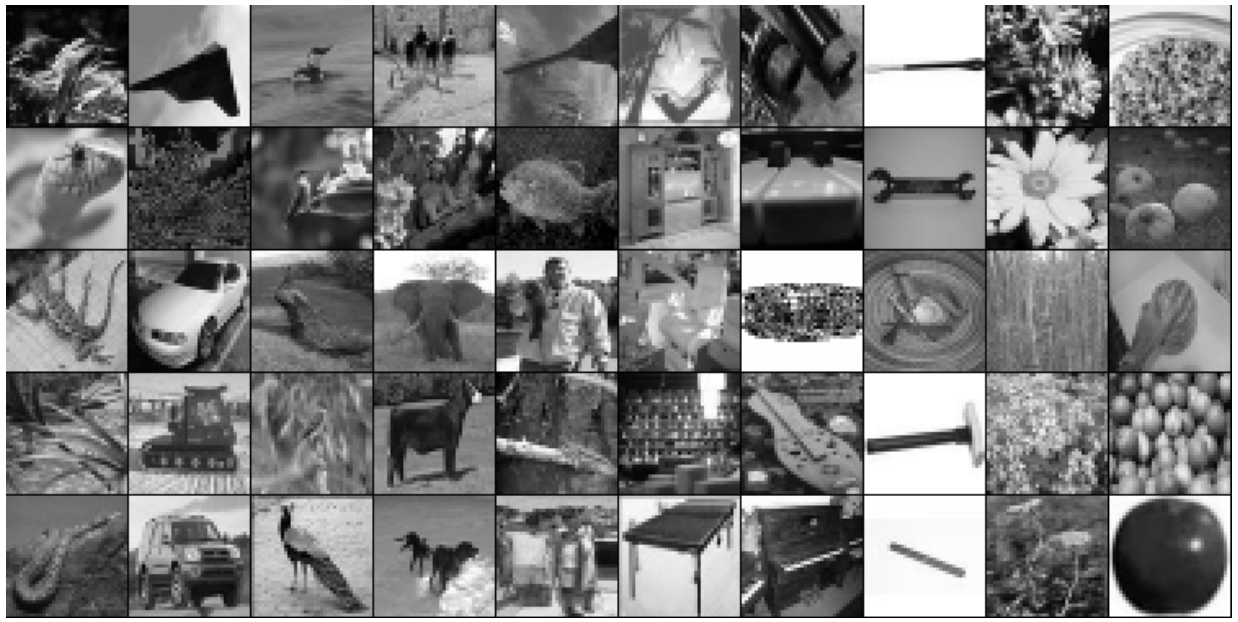
\includegraphics[width=\textwidth]{05_Understanding_deep_learning/small-ImageNet.png}
        \caption{Small-ImageNet}
        \label{fig:five over x}
    \end{subfigure}
       \caption{Three simple graphs}
       \label{fig:three graphs}
\end{figure}
\end{frame}

\begin{frame}
  \frametitle{Experimental Setting}
  \begin{itemize}
    \item They optimized feedforward neural networks: 
    \begin{itemize}
      \item With one to five hidden layers. 
      \item One thousand hidden units per layer. 
      \item Softmax logistic regression for the output. 
    \end{itemize}
    \item Cost function is the negative log-likelihood: 
    \begin{equation}
      - \log P(y|x),
    \end{equation}
    where $(x,y)$ is the (input image, target class). 
    \item NN optimized with stochastic back-propagation on mini-batches of size ten. 
    \item Learning rate is a hyperparameter that is optimized based on validation set error after a large number of updates (5 million). 
  \end{itemize}
\end{frame}

\begin{frame}
  \frametitle{Experimental setting}

  \begin{itemize}
    \item The non-linear activation functions in the hidden layers varied on: 
    \begin{itemize}
      \item The sigmoid
      \item the hyperbolic tangent,
      \item the \textit{newly proposed} softsign: 
      \begin{equation}
        \frac{x}{1 + |x|}
      \end{equation}
    \end{itemize}
  \end{itemize}

  \begin{figure}[t]
    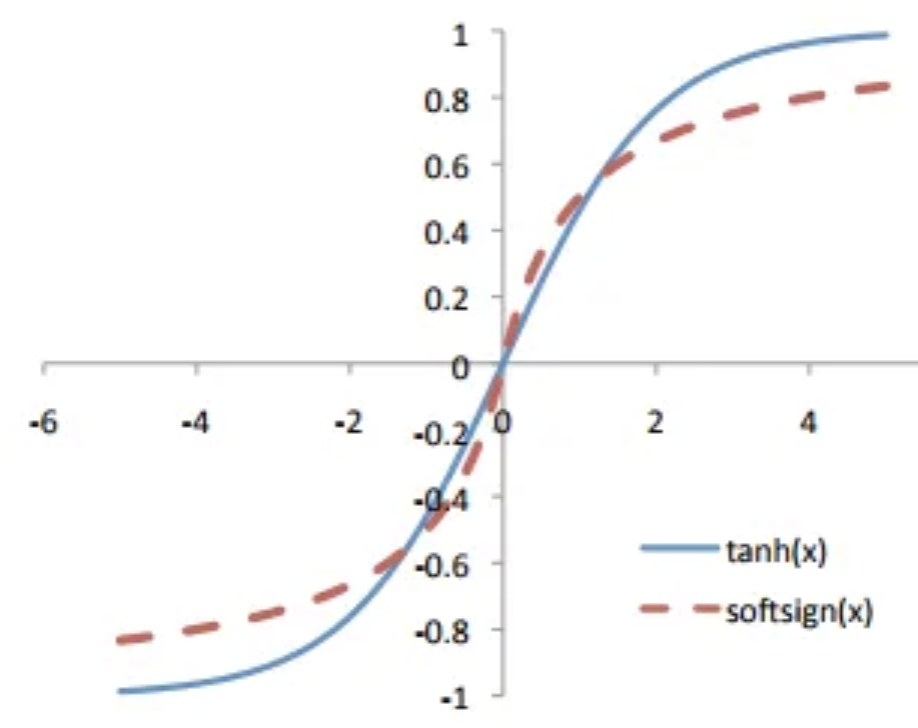
\includegraphics[height=0.4\textheight]{05_Understanding_deep_learning/softsign.png}
    \centering
\end{figure}

\end{frame}

\begin{frame}
  \frametitle{Experimental setting}

  \begin{itemize}
    \item They search for the best hyperparameters (learning rate and depth) separately for each model. 
    \item Initialization: 
    \begin{itemize}
      \item Biases to 0,
      \item the weight $W_{i j}$ at each layer with the following commonly used heuristic 
      \begin{equation}
        W_{i j} \sim U \left( - \frac{1}{\sqrt{n}}, \frac{1}{\sqrt{n}}\right), 
      \end{equation}
      where $U$ is the uniform distribution and $n$ the size of the previous layer. 
    \end{itemize}
  \end{itemize}

\end{frame}

\section{Effect of Activation Functions and Saturation During Training}

\begin{frame}
  \frametitle{Avoidable things}
\begin{itemize}
  \item Excessive saturation of activation functions (affects gradient propagation). 
  \item Overlay linear units  (will not compute something interesting).
\end{itemize}
\end{frame}

\subsection{Experiments with the Sigmoid}
\begin{frame}
  \frametitle{Experiments with the Sigmoid}

    The sigmoid non-linearity has symptomatic behaviour.
    
    \begin{itemize}
      \item Its none-zero mean that induces import singular values in the Hessian. 
      \item Saturation levels. 
    \end{itemize} 

    \textbf{Experiments considerations}

    \begin{itemize}
      \item looking at the evolution of activations during training on the Shapeset-3 x 2 data.
      
      \item  Figure \ref{fig:saturation-sigmoid-shapeset3x2} shows the evolution of the activation values (after the non- linearity) at each hidden layer during training of a deep architecture with sigmoid activation functions. 
      
      \item Layer 1 refers to the output of first hidden layer, and there are four hidden layers. 
      
      \item The graph shows the means and standard deviations of these activations. 
      
      \item These statistics along with histograms are computed at different times during learning, by looking at activation values for a fixed set of 300 test examples. 
    \end{itemize}
\end{frame}

\begin{frame}
  \frametitle{Evolution ot the activations during training}
% imgs/05_Understanding_deep_learning/saturation_sigmoid.png
\begin{figure}[t]
  \centering
  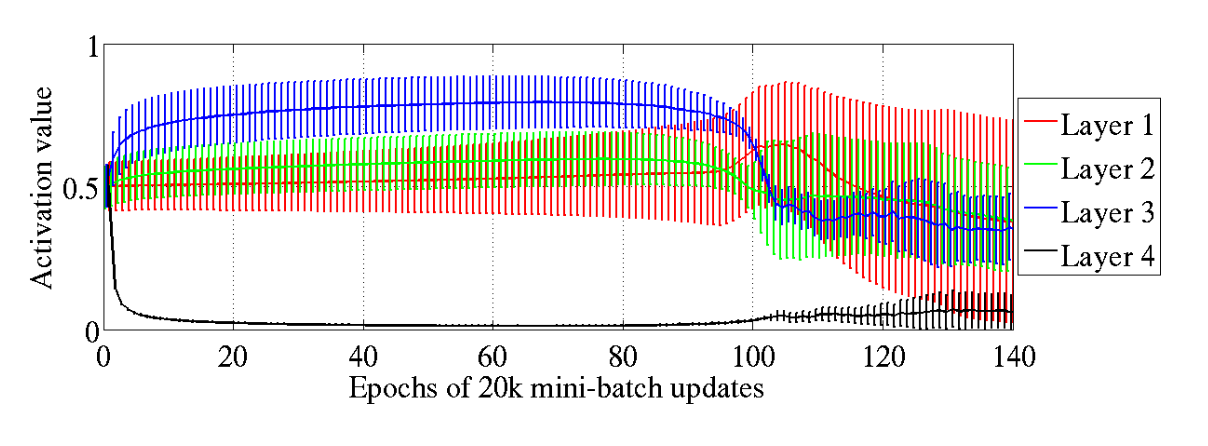
\includegraphics[height=0.6\textheight]{05_Understanding_deep_learning/saturation_sigmoid.png}
  \caption{Mean and standard deviation (vertical bars) of the activation values (output of the sigmoid) during supervised learning, for the different hidden layers of a deep architecture. The top hidden layer quickly saturates at 0 (slow- ing down all learning), but then slowly desaturates around epoch 100.}
  \label{fig:saturation-sigmoid-shapeset3x2}
\end{figure}

\end{frame}

\begin{frame}
  \frametitle{Observation}

  \begin{itemize}
    \item We see that very quickly at the beginning, all the sigmoid activation values of the last hidden layer are pushed to their lower saturation value of 0.
    
    \item the others layers have a mean activation value that is above 0.5, and decreasing as we go from the output layer to the input layer. 
    
    \item This kind of saturation can last very long in deeper networks with sigmoid activations, e.g., the depth-five model never escaped this regime during training. 
    
    \item The big surprise is that for intermediate number of hidden layers (here four), the saturation regime may be escaped. 
    
    \item The top hidden layer moves out of saturation, the first hidden layer begins to saturate and therefore to stabilize.

  \end{itemize}

\end{frame}

\begin{frame}
  \frametitle{Hypothesis}

  \begin{itemize}
    \item This behavior is due to the combination of \textbf{random initialization} and the fact that an hidden \textbf{unit output of 0 corresponds to a saturated} sigmoid since  deep networks with sigmoids but initialized from unsupervised pre-training (e.g. from RBMs) do not suffer from this saturation behavior.
    
    \item  the lower layers of the randomly initialized network computes initially is not useful to the classification task, unlike the transformation obtained from unsupervised pre-training.
    
    \item The logistic layer output $softmax(b + W h)$ might initially rely more on its biases b (which are learned very quickly) than on the top hidden activations $h$ derived from the input image (because $h$ would vary in ways that are not predictive of $y$). 
  \end{itemize}

\end{frame}


\begin{frame}
  \frametitle{Hypothesis}

  \begin{itemize}
    \item Would the error gradient wold tend to push $Wh$ towards 0, which can be achieved by pushing $h$ towards $0$. 
    
    \item  Symmetric activation functions like the hyperbolic tangent and the softsign, sitting around 0 is good because it allows gradients to flow backwards.
    
    \item pushing the sigmoid outputs to 0 would bring them into a saturation regime which would prevent gradients to flow backward and prevent the lower layers from learning useful features. 
    
    \item Eventually but slowly, the lower layers move toward more useful features and the top hidden layer then moves out of the saturation regime. However that, even after this, the network moves into a solution that is of poorer quality 
  \end{itemize}

\end{frame}


\begin{frame}
  \frametitle{Test error during online training}

  % imgs/05_Understanding_deep_learning/test_error_during_online_training.png
  \begin{figure}[t]
    \centering
    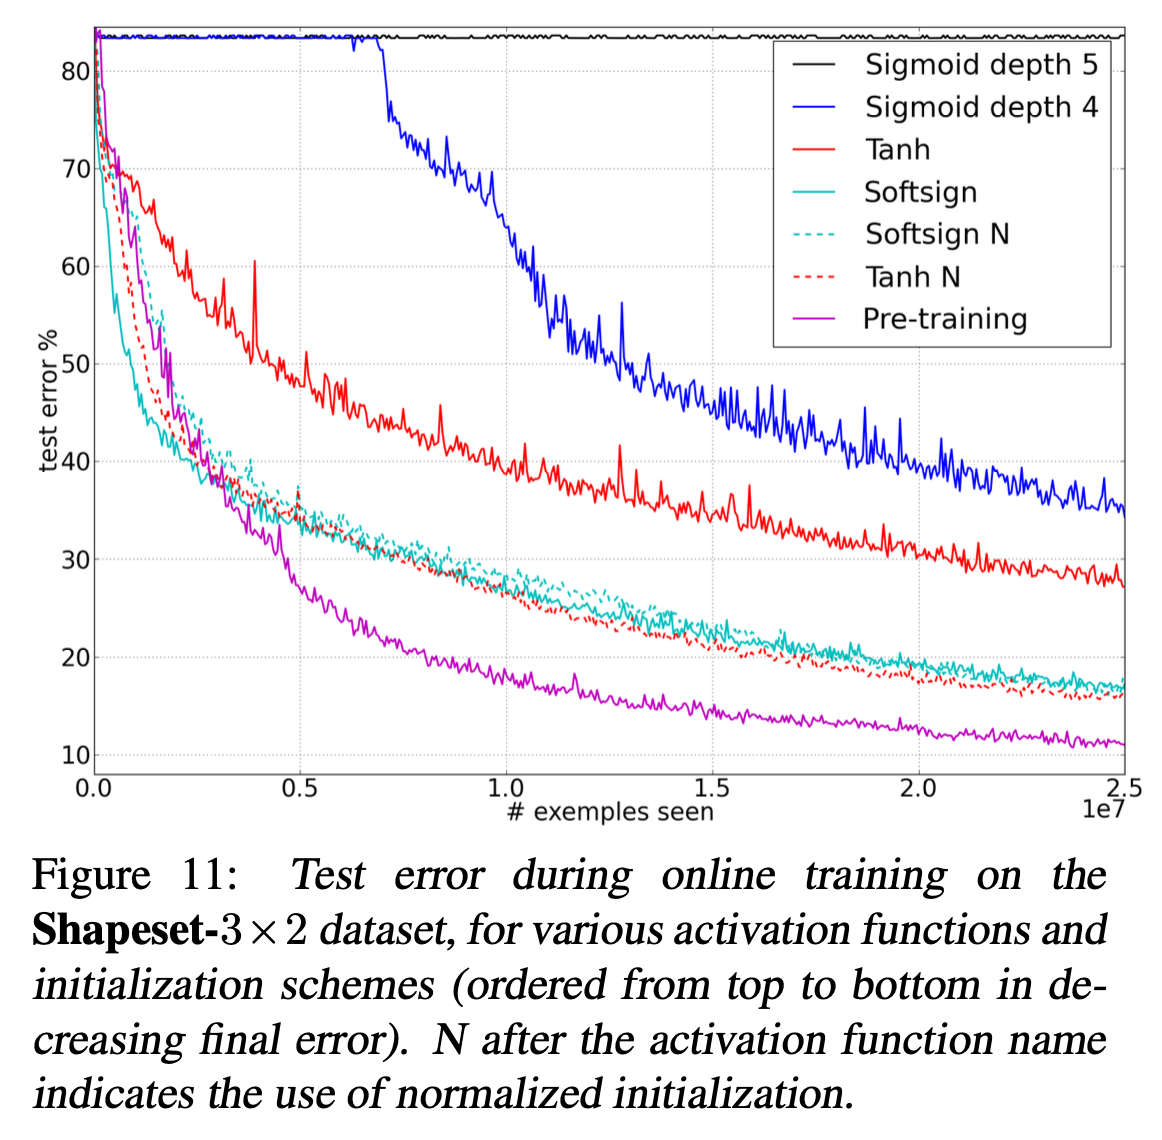
\includegraphics[height=0.8\textheight]{05_Understanding_deep_learning/test_error_during_online_training.png}
  \end{figure}
\end{frame}


\subsection{Experiments with the Hyperbolic tangent}

\begin{frame}
  \frametitle{Experiments with the Hyperbolic tangent}

  \begin{itemize}
    \item The hyperbolic tangent networks do not suffer from the kind of saturation behavior of the top hid- den layer observed with sigmoid networks, because of its symmetry around 0.
    \item With the standard weight initialization, we observe a sequentially occurring saturation phenomenon starting with layer 1 and propagating up in the network, as illustrated in Figure 3. 
    \item \textbf{Why this is happening remains to be understood.}

  \end{itemize}

\end{frame}


\begin{frame}
  \frametitle{Activation values for hiperbolic tangent and softsign}

  % imgs/05_Understanding_deep_learning/distribution_of_activation_values_for_the_hyperbolic_and_soft_sign.png
  \begin{figure}[t]
    \centering
    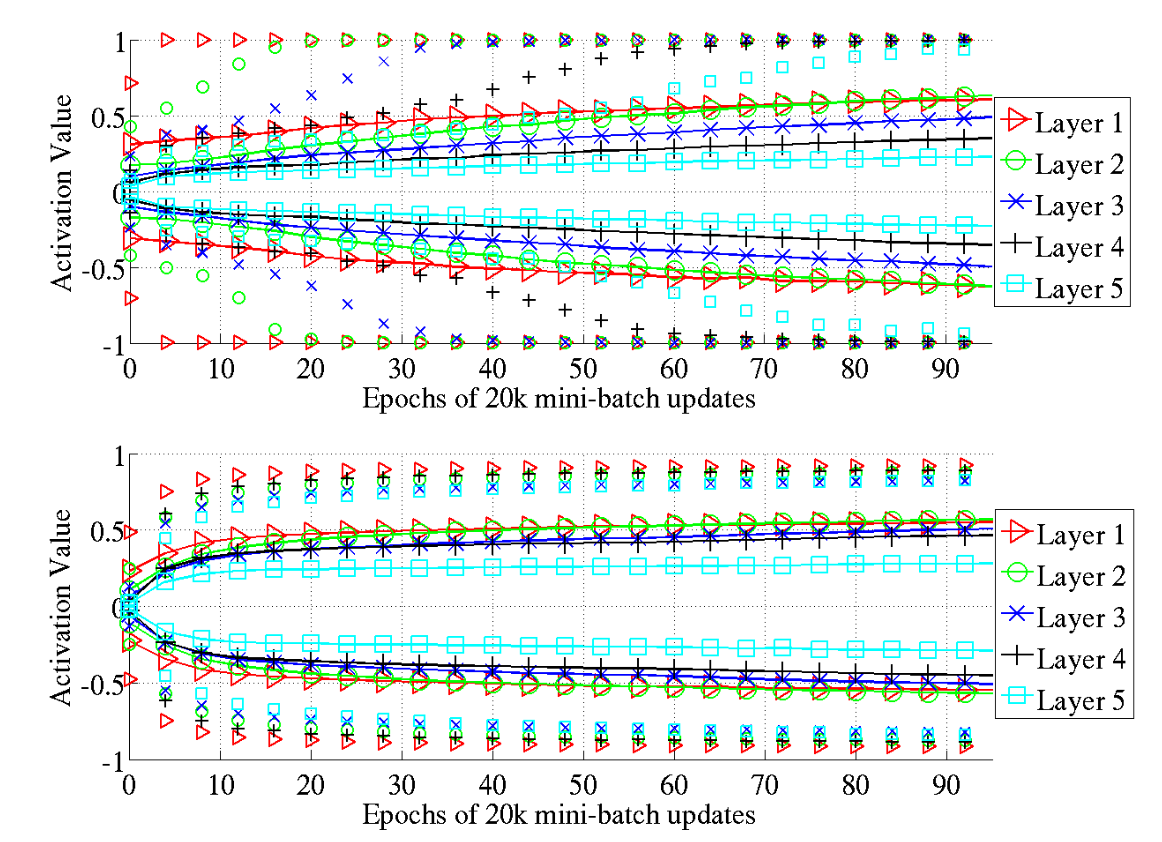
\includegraphics[height=0.5\textheight]{05_Understanding_deep_learning/distribution_of_activation_values_for_the_hyperbolic_and_soft_sign.png}
    \caption{
      Top:98 percentiles (markers alone) and standard deviation (solid lines with markers) of the distribution of the activation values for the hyperbolic tangent networks in the course of learning. We see the first hidden layer satu- rating first, then the second, etc. Bottom: 98 percentiles (markers alone) and standard deviation (solid lines with markers) of the distribution of activation values for the soft- sign during learning. Here the different layers saturate less and do so together.
    }
  \end{figure}

\end{frame}

\subsection{Experiments with the Softsign}


\begin{frame}
  \frametitle{Experiments with the Softsign}

  \begin{itemize}
    \item The softsign $x/(1+|x|)$ is similar to the hyperbolic tangent but might behave differently in terms of saturation because of its smoother asymptotes (polynomial instead of exponential). 
    
    \item We see on Figure 3 that the saturation does not occur one layer after the other like for the hyperbolic tangent. It is faster at the beginning and then slow, and all layers move together towards larger weights.
  \end{itemize}

\end{frame}

\begin{frame}
  \frametitle{Histogram of activation values at the end of the learning}
% imgs/05_Understanding_deep_learning/activation_values_at_end_of_the_learning.png
\begin{figure}[t]
  \centering
  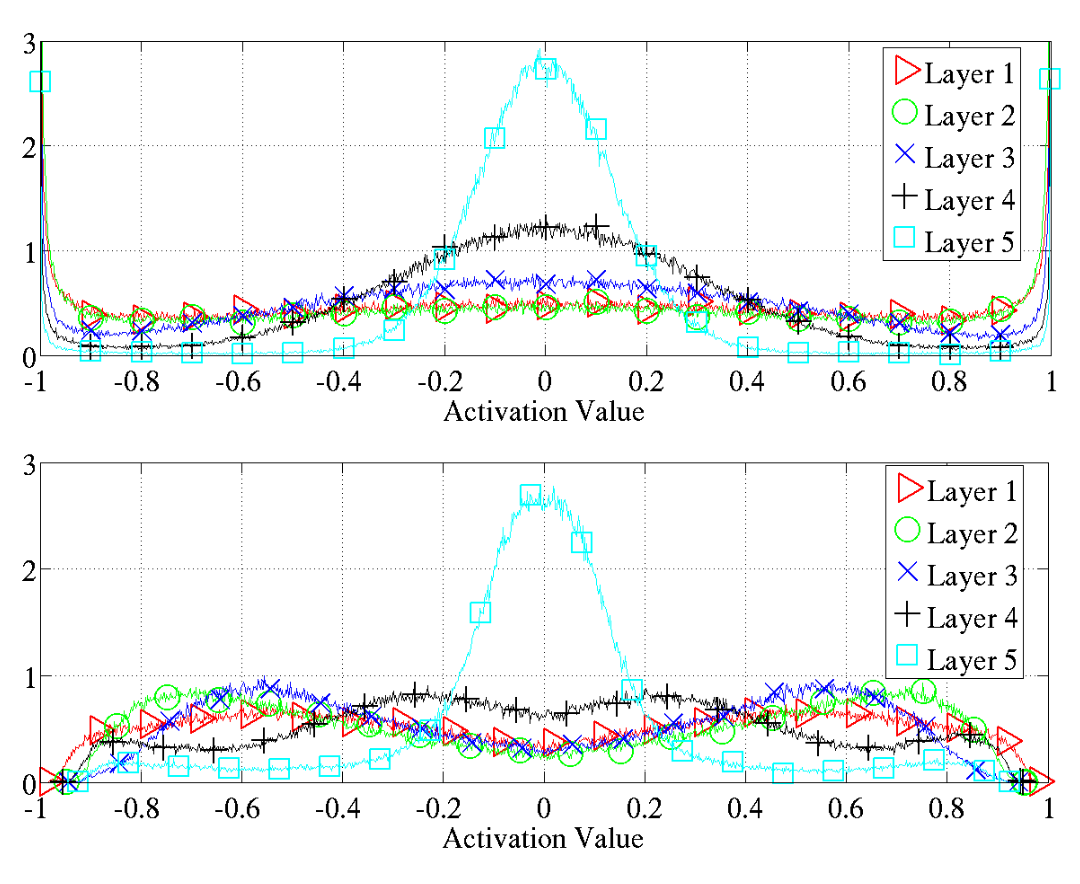
\includegraphics[height=0.5\textheight]{05_Understanding_deep_learning/activation_values_at_end_of_the_learning.png}
  \caption{
    Activation values normalized histogram at the end of learning, averaged across units of the same layer and across 300 test examples. Top: activation function is hyperbolic tangent, we see important saturation of the lower layers. Bottom: activation function is softsign, we see many activation values around (-0.6,-0.8) and (0.6,0.8) where the units do not saturate but are non-linear.
  }
\end{figure}
  
\end{frame}

\section{Studying Gradients and their Propagation}


    
\section{Randomness in neural networks: an overview}

\begin{frame}
    \frametitle{Paper information}

    \begin{itemize}
        \item Title: \textbf{Randomness in Neural Networks: An Overview}. 
        \item Authors:  Scardapane, Simone and Wang, Dianhui. 
        \item Year: 2017
        \item Number of cites: 285.
        \item \cite{randomness-in-neural-networks}
    \end{itemize}

    Drawbacks: 
    \begin{itemize}
        \item No experimental results. 
        \item Spend many sections in kernel random features we have already seen. 
    \end{itemize}
    
\end{frame}

\begin{frame}{Other articles}
    \begin{itemize}
        \item \textbf{A review on neural networks with random weights}. 
        \item Authors:  Weipeng Cao and Xizhao Wang and Zhong Ming and Jinzhu Gao.
        \item Year: 2018. 
        \item Number of cites: 308. 
        \item \cite{a-review-neural-network-with-random-weights}
    \end{itemize}
    
\end{frame}

\section{Randomness in neural networks: an overview}

\begin{frame}
    \frametitle{Main idea}

    \textbf{Randomization is cheaper than optimization}

    Three families: 
    \begin{itemize}
        \item \textit{Feedforward networks with random weights} (RW-FFN). 
        \item Random features for kernel methods.
        \item RC framework. 
    \end{itemize}

\end{frame}

\subsection{Feedforwards Networks with Random Weights}

\begin{frame}
    \frametitle{Network Architecture}

    \begin{equation}
        f(x)
        = 
        \sum_{m = 1}^B
        \beta_m h_m(x; w_m)
        = 
        \beta^T h_(x; w_1, \ldots, w_B). 
    \end{equation}
    where 
    \begin{equation}
        h_m(x) = g(a^T_m x + b_m).
    \end{equation}

    Randomness options: 
    \begin{itemize}
        \item 
    \end{itemize}
\end{frame}

\begin{frame}
    \frametitle{Randomnes in coefficients}
    Random projection: A. 

\end{frame}


\begin{frame}
    \frametitle{Randomnes in activation function}

    In the second family of methods, each function
is chosen instead as a radial basis function (RBF),
typically of Gaussian shape:

\begin{equation}
    h_m(x)
    = 
    \exp\left\{
        -a_m 
        \|x - c_m\|_2^2 
        \right\},
\end{equation}
Randomly chosen the centers $c$ and scaling factors $a_m$. 

\end{frame}


\begin{frame}
    \frametitle{Training}
    Compute $\beta^*$
    \begin{equation}
        \beta^*
        = 
        arg min_{\beta}
        \left\{
            \frac{1}{2}
            \|H \beta - y\|^2_2
            +
            \frac{\lambda}{2}
            \|\beta\|_{norm}
        \right\}
    \end{equation}

    The minimization problem admit some kinds of algebraic or parallelization optimization. 
\end{frame}
\begin{frame}
    \frametitle{Things to think!}
\begin{itemize}
    \item Why are we not training with gradient descent in the last layer?. 
    \item Why are we not training some intermediate weights?
\end{itemize}
    They are simple ideas, is weird the have not been done before. 

    \textbf{
    Are truly interesting or randomness is bounded?}

\end{frame}
\begin{frame}
    \frametitle{Universal Approximation Properties}

    \begin{itemize}
        \item The basic theoretical result on RW-FNNs was
        proven in 1995 by Igelnik and Pao, 35 with later corrections made by Li et al. 

        \item  The order of
        approximation error is $\mathcal O(C/\sqrt{B})$ , where the constant C is independent of B.

        \item There is
        always a non-zero probability of an unlucky draw
        from the probability distribution which will require
        re-initialization at some stage of approximation. Furthermore, this rapid convergence of order $1/\sqrt{B}$
        is assured only up to a given and fixed tolerance.

        \item Random-weights models
        still suffer from design choices, translated in free
        parameters, which are difficult to set optimally with
        the current mathematical framework, so practically
        they involve many trials and cross validation to find
        a good projection space, on top of the selection of
        the number of hidden [processing elements] and the
        nonlinear functions.
    \end{itemize}

\end{frame}


\begin{frame}
    \frametitle{RANDOM FEATURES FOR KERNEL
    APPROXIMATION}

    We have already delved deeper into the topic through the previous survey.
\end{frame}
\subsection{Recurrent Networks with random weights}
\begin{frame}
    \frametitle{Recurrent Networks with random weights}

    Some families: 

    Internal estate 

    \begin{equation}
        f[n] = h(W^r_i x[n] + W^r_r f[n-1] + W^r_0 y[n-1]),
    \end{equation}
    Or combination past present. 
    \begin{equation}
        f[n] =\lambda f[n] +
         (1-\lambda)h(W^r_i x[n] + W^r_r f[n-1] + W^r_0 y[n-1]),
    \end{equation}
    Tn the following steps: 
    \begin{equation}
        y[n]
        = 
        (w^0_i)^T x[n]
        + (W^0_r)^T f[n].
    \end{equation}
Training same that RW-FNN.
\end{frame}

\subsection{Theoretical properties of RC Networks}
\begin{frame}
    \frametitle{Theoretical properties of RC Networks}

    \begin{itemize}
        \item Initialization with uniform distribution in $[-1,1]$ is not a good idea in dynamic system ( could create oscillation or chaotic behaviors) due to vanish.
        \item Echo state property can be guaranteed almost always by rescaling the matrix $W$ so that its spectral radius is less than 1. (Criterio is a heuristic)
    \end{itemize}

\end{frame}



\section{Sharp analysis of low-rank kernel matrix approximations}
\begin{frame}
    \frametitle{Sharp analysis of low-rank kernel matrix approximations}

    \begin{itemize}
        \item \cite{bach2013sharp}
        \item Title: Sharp analysis of low-rank kernel matrix approximations.
        \item Author: Francis Bach.
        \item Year: 2013.
        \item Number of cites 316. 
    \end{itemize}
    
    Contribution interesting: 
    \begin{itemize}
        \item A kind of survey:
        \begin{itemize}
            \item kernel optimization, 
            \item analysis of column sampling approximation,
            \item randomized dimension reduction,
            \item theoretical analysis of predictive performance of kernel methods. 
        \end{itemize} 
        \item Number of columns in Nyström.   
    \end{itemize}
\end{frame}

\begin{frame}
    \frametitle{Contributions}

    \begin{itemize}
        \item The rank $p$ can be chosen to be linear in the degrees of freedom associated with the problem, a quantity which
        is classically used in the statistical analysis of such methods. 
        \item They present in Section 4.4 simple algorithms that have sub-quadratic running time complexity,
        and, for the square loss, provably exhibit the same predictive performance as classical algorithms than run in quadratic time (or more).
        
    \item They provide in Section 4.3 explicit examples of optimal values of the regularization parameters
and the resulting degrees of freedom, as functions of the decay of the eigenvalues of the kernel matrix, shedding some light in the joint computational/statistical trade-offs for choosing a
good kernel.
\item  They show that with kernels with fast spectrum decays (such as the
Gaussian kernel), computational limitations may prevent exploring the relevant portions of the
regularization paths, leading to underfitting.
    \end{itemize}
\end{frame}

\begin{frame}
    \frametitle{Degrees of freedom}

    Degrees of freedom: 
    \begin{equation}
        tr K^2(K + n \lambda I)^{-2}.
    \end{equation}
    They  define \textit{maximal marginal degrees of freedom $d$}
    as 
    \begin{equation}
        d 
        = 
        n \|
        diag( K(K + n \lambda I)^{-1}
        \|_\infty. 
    \end{equation}
    $d$ provides an upper-bound on the regular degrees of freedom.
\end{frame}


\begin{frame}
    \frametitle{Predictive performance of column sampling}

    Consider sampling p columns (without replacement) from the original n columns. We consider
the column sampling approximation and provide sufficient conditions (a lower-bound on $p$) to obtain the same predictive performance than with the full kernel matrix.

\end{frame}

\begin{frame}
    \begin{figure}[t]
        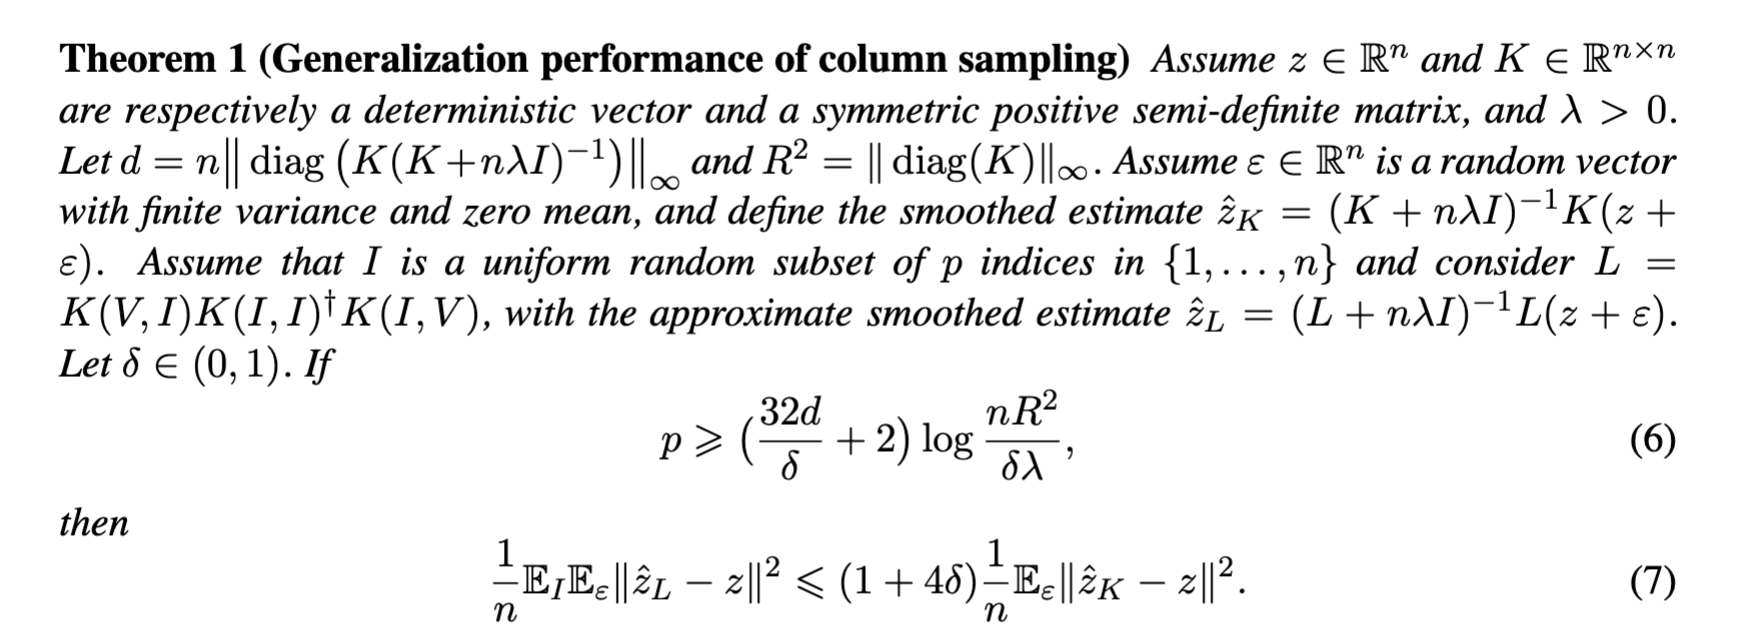
\includegraphics[width=1.05\textwidth]{11-kernel-survey/theorem_1.png}
        \centering
    \end{figure}
\end{frame}


\begin{frame}
    \frametitle{Some observations}

    \begin{itemize}
        \item Provides a relative approximation guarantee (small values of $\delta$). 
        \item $p$ seen to by large in practise $\dots$
        \item Avoiding terms in $1/\lambda$. 
        \item Regularization effects.  
    \end{itemize}
\end{frame}

\begin{frame}
    \frametitle{Optimal choice of the regularization parameter}

    \begin{itemize}
        \item Based on eigenvalues and $n$.
        \item Provide some simulations. 
    \end{itemize}
\end{frame}
\section{ Fast and scalable polynomial kernels via explicit feature maps}
\begin{frame}
    \frametitle{Fast and scalable polynomial kernels via explicit feature maps}
\begin{itemize}
    \item \cite{fast-and-scalable-polynomial-kernels}
    \item Cited by 296. 
    \item Year 2013. 
\end{itemize}

\textbf{Util for us}
\begin{itemize}
    \item Good approach for polynomial kernel 
    \begin{equation}
        k(x,y)
        = 
        (\langle x, y  \rangle + c)^p. 
    \end{equation}
\end{itemize}


\end{frame}


\begin{frame}
    \frametitle{Content}
    \begin{itemize}
        \item They introduce a fast and scalable randomized tensor product technique for approximating polynomial kernels,
        
        \item Accelerating the training of kernel machines. 
        
        \item By exploiting the connection between tensor product and fast convolution of Count Sketches, our approximation algorithm works in time O(n(d+D log D)) for n training samples in d-dimensional space and D random features.
    \end{itemize}
    

\end{frame}


\begin{frame}
    \frametitle{Objetivos semana siguiente}

    - Disminuir coste computacional SVM (Kernel ridge, GP)
    - Deep Redes neuronales 

    Ideas simplificación: 
    -  RF
    - Nyström  
----------------
Contar todas las cosas y hacer experimentos. 


\end{frame}
\begin{frame}
    \frametitle{Large scale machine Learning}

    \begin{itemize}
        \item Cite \cite{wang2020survey},
        \item cited by 60. 
    \end{itemize}

\end{frame}

\begin{frame}{Article sections}
    \begin{figure}[t]
        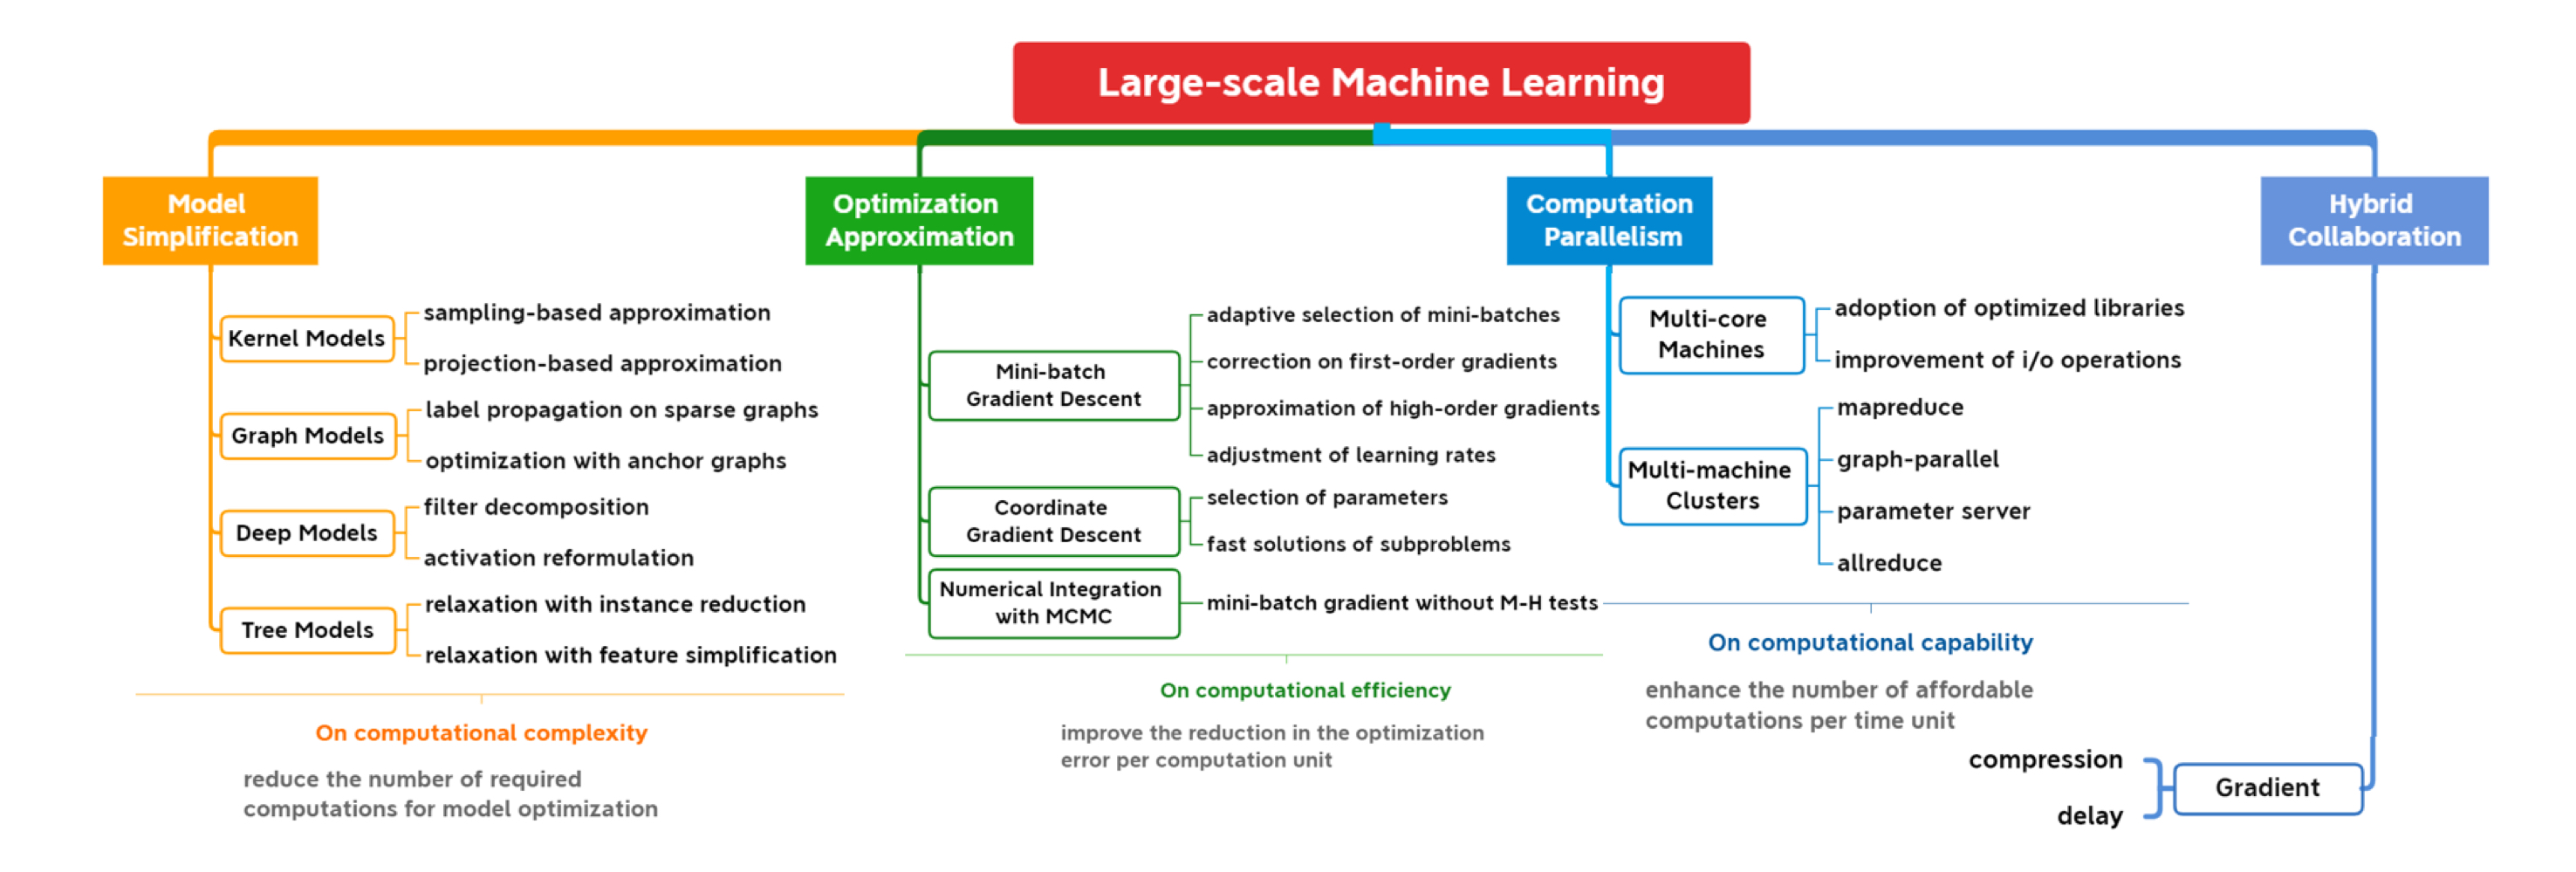
\includegraphics[width=\textwidth]{11-kernel-survey/large-scale-machine-learning.jpeg}
        \centering
    \end{figure}


\end{frame}

%%%%%%%%%%%%%%%%%%%%%%%%%%%%%%%%%

% Import bibliography from file sample.bib
\begin{frame}[t, allowframebreaks]
\frametitle{References}
\bibliography{../../bibliography}
\end{frame}

\end{document}